%% ============================================================================
%% When Semantic Caches Lie
%% Independent research paper by Sunny Patel
%% Diamond-standard preamble (XCharter text + newtxmath, biblatex/biber, booktabs)
%% Compile: latexmk -pdf -cd main.tex   (biber auto-detected from biblatex)
%% ============================================================================
\documentclass[11pt,letterpaper]{article}

%% --- Math first (amsmath/mathtools before newtxmath, per newtx docs) ---------
\usepackage{amsmath}
\usepackage{mathtools}

%% --- Fonts: XCharter text + matched Charter math (single math package) -------
%% newtxmath provides the AMS symbol set, so amssymb is intentionally NOT loaded
%% (loading it clashes with newtxmath over \Bbbk).
\usepackage[T1]{fontenc}
\usepackage[utf8]{inputenc}
\usepackage{XCharter}
\usepackage[charter]{newtxmath}

%% --- Microtypography ---------------------------------------------------------
% Protrusion (character protrusion into the margin) is the larger visual win and is
% cheap; font expansion is disabled because generating expanded Type1 instances for the
% many newtx symbol fonts is pathologically slow at this font count.
\usepackage[protrusion=true,expansion=false,final]{microtype}

%% --- Geometry & spacing ------------------------------------------------------
\usepackage[margin=1in]{geometry}

%% --- Tables ------------------------------------------------------------------
%% Numbers are pre-formatted to a fixed number of decimals by the table-generation
%% code and right-aligned, which aligns the decimal points cleanly. (siunitx's S
%% columns interact pathologically slowly with the newtx math fonts in this toolchain.)
\usepackage{booktabs}
\usepackage{threeparttable}

%% --- Graphics & figures ------------------------------------------------------
\usepackage{graphicx}
\usepackage[dvipsnames]{xcolor}
\usepackage[labelsep=endash,font=small]{caption}
\usepackage{subcaption}

%% --- Lists & quotes ----------------------------------------------------------
\usepackage{enumitem}
\setlist[itemize]{itemsep=4pt,topsep=4pt}
\setlist[enumerate]{itemsep=4pt,topsep=4pt}
\usepackage[american]{babel}
\usepackage{csquotes}

%% --- Hyperlinks (bare, then \hypersetup) then cleveref ----------------------
\usepackage{hyperref}
\definecolor{linknavy}{rgb}{0.10,0.20,0.45}
\definecolor{citegreen}{rgb}{0.00,0.34,0.20}
\definecolor{urlblue}{rgb}{0.10,0.22,0.55}
\hypersetup{
  colorlinks=true,
  linkcolor=linknavy,   % internal cross-references (sections, figures, equations)
  citecolor=citegreen,  % citations
  urlcolor=urlblue,     % external links
  breaklinks=true,
  pdftitle={When Semantic Caches Lie: False Hits, Downstream Cost, and Calibration},
  pdfauthor={Sunny Patel},
  pdfkeywords={semantic caching, large language models, embedding models, false-hit rate, calibration, retrieval}
}
\usepackage{cleveref}

%% --- Bibliography ------------------------------------------------------------
\usepackage[backend=biber,style=numeric-comp,sorting=nyt,sortcites=true,
            maxbibnames=99,giveninits=true,url=false,doi=true,eprint=true]{biblatex}
\addbibresource{references.bib}

%% --- Shared macros and notation ----------------------------------------------
% Shared macros and notation.

% A visible placeholder for a number to be filled from the final results.
% Every \pending must be resolved before submission (grep for it).
\newcommand{\pending}[1]{{\bfseries[#1]}}

% Notation
\newcommand{\simfun}{s}            % similarity score
\newcommand{\thr}{\tau}            % decision threshold
\newcommand{\query}{q}             % an incoming query
\newcommand{\cached}{c}            % a cached entry
\newcommand{\emb}[1]{\mathbf{e}_{#1}}
\DeclareMathOperator{\cossim}{cos}
\newcommand{\fhr}{\textsc{fhr}}    % false-hit rate
\newcommand{\prauc}{\textsc{pr}\text{-}\textsc{auc}}
\newcommand{\rocauc}{\textsc{roc}\text{-}\textsc{auc}}
\newcommand{\Real}{\mathbb{R}}


%% --- Widow/orphan control ----------------------------------------------------
\widowpenalty=10000
\clubpenalty=10000

%% --- Title -------------------------------------------------------------------
\title{\bfseries When Semantic Caches Lie:\\ False Hits, Downstream Cost, and Calibration\\[2pt]
\large in Embedding-Based Caching for Large Language Models}
\author{Sunny Patel%
\thanks{Copyright \textcopyright{} 2026 Sunny Patel. All rights reserved. This manuscript and
its figures are the author's intellectual property; see the project license.
{ORCID}: \href{https://orcid.org/0009-0005-3863-7642}{0009-0005-3863-7642}.
Correspondence: \texttt{sunnypatel124555@gmail.com}. Website: \url{https://www.sunnypatel.net}.
Code and data: \url{https://github.com/sunnypatell/semantic-cache-reliability}.}\\[2pt]
\small Independent Researcher, Toronto, Canada \\[1pt]
\small \href{https://orcid.org/0009-0005-3863-7642}{ORCID 0009-0005-3863-7642}}
\date{}

\begin{document}
\maketitle

\begin{abstract}
\noindent
A semantic cache reuses a stored answer whenever a new prompt's embedding is close
enough to an earlier one, trading a model call for a lookup. The threshold that governs
this trade also governs a quiet failure: a \emph{false hit}, where the cache returns a
confident answer to a prompt the stored answer does not fit. We argue that the property
a cache needs, whether one prompt's answer is valid for another, is not the embedding
similarity it can measure, and we study the gap between them. Grounding
cache-equivalence in human-labeled prompt pairs rather than in embedding geometry, we
map the false-hit rate of six sentence-embedding models across three domains and the
full range of thresholds, with bootstrap confidence intervals, and report the operating
points deployments care about. We then inject false hits into retrieval and generation
to measure what they cost once served, and we calibrate the threshold to that cost.
\pending{One- or two-sentence headline finding, filled from final results.} A cost-aware
policy that ties the operating point to the measured penalty of a false hit improves the
cost--coverage frontier over fixed and correctness-bounding thresholds, and it transfers
across domains. The results caution against trusting a single similarity threshold, and
they give practitioners a principled way to set one.
\end{abstract}

\section{Introduction}
\label{sec:intro}

A semantic cache answers a new prompt with a stored response whenever the new prompt
looks close enough to one the system has already served. Closeness is judged in an
embedding space: the cache encodes the incoming query, finds its nearest stored
neighbor, and returns the neighbor's answer when their cosine similarity clears a
threshold $\thr$. The appeal is obvious. A served hit skips a model call, so a cache
that fires often turns the dominant cost of an \mbox{LLM} service, inference, into a
lookup~\cite{bang2023gptcache,gill2024meancache}. Production systems now ship semantic
caches by default, and recent work has pushed their hit rates higher and added online
guarantees on correctness~\cite{schroeder2025vcache,wang2025categoryaware}.

The threshold hides a hard decision. Set it low and the cache fires often, paying back
its keep, but it also begins to serve answers to prompts that only resemble an earlier
one. Set it high and those mistakes vanish, along with most of the savings. The mistake
itself is quiet. When the cache returns a stored answer to a prompt it does not actually
fit, nothing errors and nothing logs; the user simply receives a confident, wrong
reply. We call this a \emph{false hit}, and it is the failure mode this paper measures.

The difficulty is that embedding similarity and answer reuse are not the same property.
Two prompts can be near-identical in wording yet require opposite answers, as ``what are
the strengths of this design'' and ``what are the weaknesses of this design'' do; two
others can share almost no words yet take the same answer. Similarity is what the cache
can see. \emph{Cache-equivalence}, the question of whether one prompt's stored answer is
valid for another, is what it needs. Prior work has largely optimized the first as a
proxy for the second: it tunes thresholds, learns them online from correctness
feedback~\cite{schroeder2025vcache}, specializes them by query
category~\cite{wang2025categoryaware}, or sharpens the embedding
itself~\cite{gill2025advancing}. What the literature has not done is measure how often
the proxy fails when it is not under attack, chart how that failure rate moves with the
embedding model and the domain, follow it into the quality of the task the cache serves,
or turn the measurement into an operating point that accounts for what a false hit
actually costs. The one adversarial study of these caches shows the proxy can be broken
on purpose~\cite{zhang2026keycollision}; we ask how often it breaks on its own.

This paper answers that question with a measurement study and a calibration method built
on it. We separate cache-equivalence from textual similarity and label it directly,
drawing on human-annotated pair corpora whose judgments encode same-meaning rather than
word overlap~\cite{zhang2019paws,wang2019glue,dolan2005mrpc}. On this footing we measure
the false-hit rate of six widely used sentence
embeddings~\cite{reimers2019sentencebert,wang2022e5,xiao2023cpack} across three domains
and the full range of thresholds, report it with bootstrap confidence intervals, and
read off the operating points a practitioner reasons about: how much of the traffic a
cache can serve while holding its error below a ceiling, and how clean it can be while
still reusing a target share of genuinely reusable answers. We then inject false hits
into downstream retrieval and generation to measure what they cost once served, and we
use that cost to calibrate the threshold. The resulting policy minimizes expected cost
under the measured, asymmetric penalty of a false hit, and it transfers across models
and domains without the per-prompt online feedback that earlier correctness-bounding
methods require.

Our findings are not reassuring for the default of trusting a single similarity threshold.
On adversarial paraphrases the strongest embedding reaches a \rocauc{} of only $0.67$, and a
lexical baseline outscores every neural encoder, because the surface-form insensitivity that
makes an embedding useful is exactly what blinds it to a word-scrambled near-duplicate.
Holding the false-hit rate under one percent caps coverage near nine percent on the easiest
domain and under one percent on the others. Downstream, a false hit is nearly as costly when it
corrupts the retrieved context as when it corrupts the final answer, because the reader rarely
recovers from a wrong premise; what softens the damage is a milder corruption, not an earlier
position in the pipeline. A fixed similarity threshold proves
catastrophic under a realistic false-hit penalty, costing several times the price of not
caching at all, while a threshold calibrated to the measured penalty recovers near-baseline
cost and adapts to each domain's difficulty. Such a threshold transfers only in the
conservative direction: a value tuned on an easy domain backfires when reused on a hard one.

\paragraph{Contributions.}
\begin{itemize}
  \item A \emph{cache-equivalence} construct that separates ``safe to reuse the stored
        answer'' from ``looks similar,'' together with a labeling protocol that grounds
        it in human judgments rather than embedding geometry (\cref{sec:setup}).
  \item The first systematic map of benign false-hit economics for embedding caches:
        false-hit rate and coverage across six encoders, three domains, and all
        thresholds, with bootstrap confidence intervals and the operating points that
        matter in deployment (\cref{sec:results}).
  \item A measurement of the downstream cost of a false hit, obtained by controlled
        fault injection into retrieval and generation, broken down by task and by the
        cache's position in the pipeline (\cref{sec:downstream}).
  \item A cost-aware threshold-calibration policy that ties the operating point to the
        measured cost of a false hit. It exposes that a fixed default is catastrophic under a
        realistic penalty, matches a correctness-bounding baseline without a hand-set error
        target, and reveals that thresholds transfer across domains only in the conservative
        direction (\cref{sec:calibration}).
\end{itemize}

All code, the labeled data, and the exact commands that regenerate every number and
figure are released with the paper.


\section{What a cache must decide}
\label{sec:setup}

\subsection{The decision and its failure mode}
A semantic cache holds a set of prompt--response pairs. When a query $\query$ arrives,
the cache encodes it to a vector $\emb{\query}$, retrieves the nearest stored entry
$\cached$ with vector $\emb{\cached}$, and computes the cosine similarity
$\simfun = \cossim(\emb{\query}, \emb{\cached})$. If $\simfun \ge \thr$ the cache serves
$\cached$'s stored response; otherwise the query falls through to the model. The single
free parameter is the threshold $\thr$.

A served query is a \emph{hit}. A hit is \emph{true} when the stored response is a valid
answer to $\query$ and \emph{false} when it is not. The quantity we track is the
false-hit rate among served queries,
\begin{equation}
  \fhr(\thr) \;=\; \Pr\!\left[\,\text{not equivalent} \;\middle|\; \simfun \ge \thr\,\right]
            \;=\; 1 - \operatorname{precision}(\thr),
  \label{eq:fhr}
\end{equation}
reported together with \emph{coverage}, the fraction of queries the cache serves at
$\thr$. Coverage is the benefit and $\fhr$ is the silent cost, and the threshold trades
one for the other. \Cref{tab:notation} collects the notation used throughout.

\begin{table}[t]
  \centering
  \caption{Notation used throughout the paper.}
  \label{tab:notation}
  \small
  \begin{tabular}{@{}r@{\ \ }l@{\hspace{2.2em}}r@{\ \ }l@{}}
    \toprule
    Symbol & Meaning & Symbol & Meaning \\
    \midrule
    $\query$ & incoming query (prompt)            & $\fhr(\thr)$ & false-hit rate, $1-\text{precision}$ \\
    $\cached$ & nearest stored entry              & $\cov(\thr)$ & coverage, fraction served \\
    $\emb{\cdot}$ & unit embedding of a prompt     & $\cfh$ & cost of a false hit (model calls) \\
    $\simfun$ & cosine $\cossim(\emb{\query},\emb{\cached})$ & $\cost(\thr)$ & expected cost per query \\
    $\thr$ & threshold; serve iff $\simfun\ge\thr$ & $N$ & number of queries \\
    $\mathrm{TP},\mathrm{FP}$ & true / false hits at $\thr$ & $\prauc,\rocauc$ & threshold-free separability \\
    \bottomrule
  \end{tabular}
\end{table}

\subsection{Cache-equivalence is not similarity}
The label in \cref{eq:fhr} is the crux. We define two prompts as \emph{cache-equivalent}
when the stored response to one is a factually and logically valid answer to the other,
so that serving it requires no regeneration. This is a property of answers, not of
surface form. It is distinct from cosine similarity, which is all the cache can observe,
and the gap between the two is precisely where false hits live: a pair that scores high
yet is not equivalent is a false hit waiting to happen.

Because cache-equivalence is a human judgment, we ground it in human-labeled data rather
than in the embedding geometry we are auditing. We use three public pair corpora whose
annotations encode same-meaning or same-intent (\cref{tab:datasets}). Quora Question
Pairs labels whether two questions are duplicates, and duplicate questions are, by
construction, questions that should receive the same answer~\cite{wang2019glue}. The
Microsoft Research Paraphrase Corpus labels sentential equivalence in a more formal,
news register~\cite{dolan2005mrpc}. \mbox{PAWS} is the decisive case: its pairs are
constructed to share almost all of their words while frequently differing in meaning, so
it isolates the prompts that look identical to a cache yet must not share an
answer~\cite{zhang2019paws}. Treating question-duplication and paraphrase as proxies for
answer-equivalence is defensible but imperfect, and we return to the limits of the proxy
in \cref{sec:threats}.

\begin{table}[t]
  \centering
  \begin{threeparttable}
    \caption{The three labeled domains. Base rate is the fraction of pairs labeled
      cache-equivalent. \mbox{PAWS} pairs are built to maximize lexical overlap, which
      makes it the hardest case for a similarity cache.}
    \label{tab:datasets}
    \begin{tabular}{l l r r}
      \toprule
      Domain & Source & Pairs & Base rate \\
      \midrule
      Questions (\textsc{qqp})   & Quora Question Pairs       & 2500 & 0.36 \\
      News (\textsc{mrpc})       & MS Research Paraphrase     & 2500 & 0.68 \\
      Adversarial (\textsc{paws}) & Word-scrambled paraphrase & 2500 & 0.44 \\
      \bottomrule
    \end{tabular}
  \end{threeparttable}
\end{table}

\subsection{Encoders}
We measure six sentence embedding models that span the sizes and families a practitioner
would actually reach for: \texttt{all-MiniLM-L6-v2} and \texttt{all-mpnet-base-v2} from
the Sentence-Transformers family~\cite{reimers2019sentencebert,song2020mpnet}, the small
and large \mbox{E5} models~\cite{wang2022e5}, and the base and large \mbox{BGE}
models~\cite{xiao2023cpack}. Each model is used in its recommended configuration for
symmetric similarity, and exact identifiers and revisions are recorded in the model
cards (\cref{app:modelcards}). A lexical \mbox{TF-IDF} cosine serves as a non-neural
control, fit unsupervised on word unigrams and bigrams of the pair text with no use of the
labels, which isolates how much of the cache's behavior comes from learned semantics rather
than word overlap. We additionally evaluate a cross-encoder that scores each pair jointly
rather than embedding the two prompts independently; it cannot serve as an indexable cache,
but it bounds what a verification layer can achieve (\cref{sec:results}).

\subsection{Metrics}
Two prompts in a labeled pair give one similarity score and one equivalence label, so a
domain--encoder combination yields a set of $(\,\text{label},\, \simfun\,)$ observations.
From these we report threshold-free separability first, because it does not depend on a
chosen operating point: the area under the precision--recall curve ($\prauc$), which is
informative under the class imbalance typical of cache traffic, and the area under the
\mbox{ROC} curve ($\rocauc$) as a secondary summary. We then report the two operating
points a deployment cares about. \emph{Coverage at a false-hit ceiling} answers ``if the
cache may serve a wrong answer no more than once in a hundred, how much traffic can it
serve?'' \emph{Precision at a recall target} answers its dual, ``if the cache must reuse
at least this share of genuinely reusable answers, how clean can it be?'' Cosine scores
are not comparable across encoders, so all cross-encoder comparison uses the
threshold-free metrics, and per-encoder thresholds are calibrated separately
(\cref{sec:calibration}).

\subsection{Statistics}
Every reported quantity carries a $95\%$ bias-corrected and accelerated bootstrap
confidence interval over pairs~\cite{efron1987bootstrap,efron1993bootstrap}, which suits
the skewed sampling distribution of a rare-event rate better than a normal
approximation. Differences between methods on a shared set use a paired bootstrap, and
the many comparisons across encoders, domains, and thresholds are corrected for multiple
testing with the Benjamini--Hochberg procedure~\cite{benjamini1995fdr}; we report effect
sizes alongside every test~\cite{dror2018hitchhiker}. The analysis plan, the primary
metric, and the sample sizes were fixed before the main run in a plan released with the code
(\cref{app:prereg}).


\section{How often the proxy fails}
\label{sec:results}

We report separability first, because it does not depend on a chosen threshold, then the
false-hit/coverage trade-off (\cref{fig:frontier}), the score distributions that explain it,
and the operating points a deployment would actually run.

\begin{figure}[t]
  \centering
  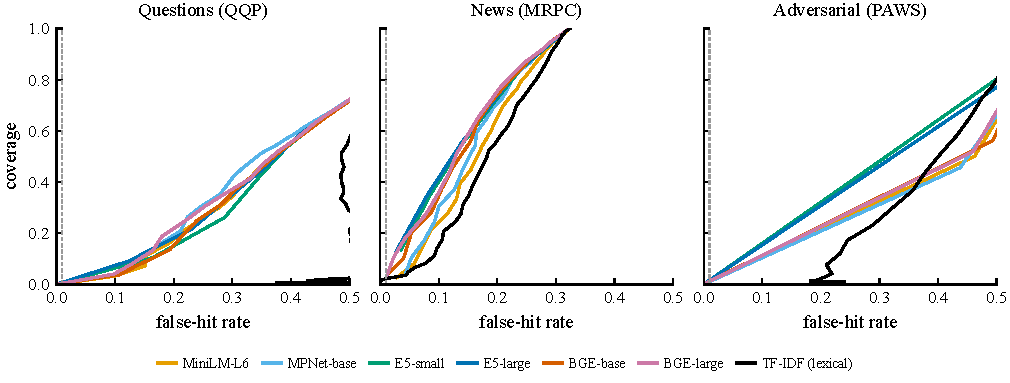
\includegraphics[width=\linewidth]{figures/fig_frontier}
  \caption{The cost of safety. Each curve sweeps the similarity threshold for one encoder;
    the vertical axis is coverage (the fraction of queries served) and the horizontal axis
    is the false-hit rate among those served. Up-and-to-the-left is better. The dashed line
    marks a $1\%$ false-hit ceiling. On questions and news, low-error operation costs most
    of the coverage; on the adversarial domain (right) the frontier collapses toward the
    diagonal, where coverage can be bought only by accepting an almost equal rate of wrong
    answers. Bands are $95\%$ bootstrap intervals.}
  \label{fig:frontier}
\end{figure}

\subsection{Separability across models and domains}
\label{sec:results-auc}
\Cref{fig:heatmap} and \cref{tab:separability} summarize threshold-free separability as
\prauc{} for every encoder--domain pair. Three patterns hold. First, the domain matters
more than the model. For a fixed encoder the spread of \prauc{} across domains is wide,
$0.62$ to $0.90$ for E5-large, while the spread across the six neural encoders within a
fixed domain is narrow, $0.54$ to $0.62$ on the adversarial set. Second, the adversarial
domain is close to unsolved: the best encoder reaches \prauc${}=0.62$ on \mbox{PAWS} against
a base rate of $0.44$, and its \rocauc{} of $0.67$ is barely above the $0.5$ of chance.
Scale buys little: moving from E5-small to E5-large raises \mbox{PAWS} \prauc{} by $0.08$,
and the \mbox{BGE} base-to-large gain is $0.04$. Third, and most telling, the lexical control
inverts the order. \mbox{TF-IDF} trails the neural encoders badly on questions, $0.49$
against $0.74$ to $0.78$, yet on the adversarial domain it \emph{outscores every neural
encoder}, $0.66$ against at most $0.62$. Word-scrambling defeats the semantics the neural
models encode, while the bigram structure the lexical model reads survives it. The very
property that makes an embedding useful, insensitivity to surface form, is what makes it
blind to an adversarial paraphrase.

\begin{figure}[t]
  \centering
  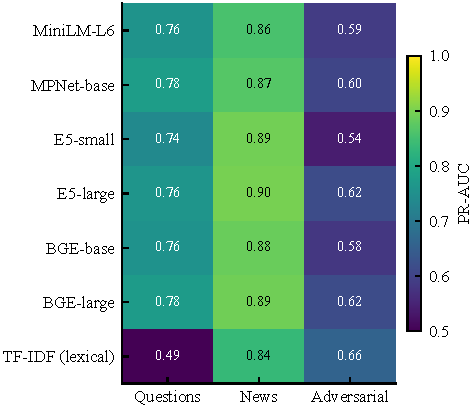
\includegraphics[width=0.82\linewidth]{figures/fig_heatmap}
  \caption{Threshold-free separability (\prauc{}) for each encoder and domain. Higher is
    better; the base rate of equivalent pairs is $0.36$ (questions), $0.68$ (news), and
    $0.44$ (adversarial). The adversarial column stays near the floor for every encoder.}
  \label{fig:heatmap}
\end{figure}

% Generated from results/reliability_summary.csv by experiments/make_tables.py
% Placeholder; regenerated by experiments/make_tables.py from results/reliability_summary.csv.
\begin{table}[t]
  \centering
  \begin{threeparttable}
    \caption{Threshold-free separability (\prauc{}) with $95\%$ bootstrap intervals, for
      every encoder and domain (placeholder; regenerated from results).}
    \label{tab:separability}
    \begin{tabular}{l c c c}
      \toprule
      Encoder & Questions & News & Adversarial \\
      \midrule
      MiniLM-L6 & -- & -- & -- \\
      \bottomrule
    \end{tabular}
  \end{threeparttable}
\end{table}


\subsection{The false-hit/coverage frontier}
\label{sec:results-frontier}
\Cref{fig:frontier} reads the same data as an operating curve. To hold the false-hit rate
under $1\%$, a deployment must move far up the threshold, and coverage falls with it. On
news the best encoder (E5-large) serves about $9\%$ of traffic at a $1\%$ ceiling; on
questions it serves under $1\%$; on the adversarial domain it serves essentially nothing.
Loosening the ceiling to $5\%$ raises news coverage to about $24\%$ but leaves questions
under $3\%$ and the adversarial domain under $1\%$. The news frontier is the most forgiving
because its pairs are the least lexically confusable; the adversarial frontier is the
warning, because it is the case a real cache meets whenever two prompts differ in a small
but decisive word.

\subsection{Why: the grey zone}
\label{sec:results-greyzone}
\Cref{fig:scores} shows where the failure comes from. For \mbox{BGE-large}, the similarity
scores of equivalent and non-equivalent pairs are well separated on questions but pile into
the same narrow, high band on the adversarial domain. On \mbox{PAWS} the median similarity
of equivalent and non-equivalent pairs differs by only $0.011$, both above $0.97$, against a
gap of $0.19$ on questions; no threshold can divide distributions that overlap this tightly.
A cache cannot act on a distinction its encoder does not represent, and on adversarial
near-duplicates the encoder does not represent it.

\begin{figure}[t]
  \centering
  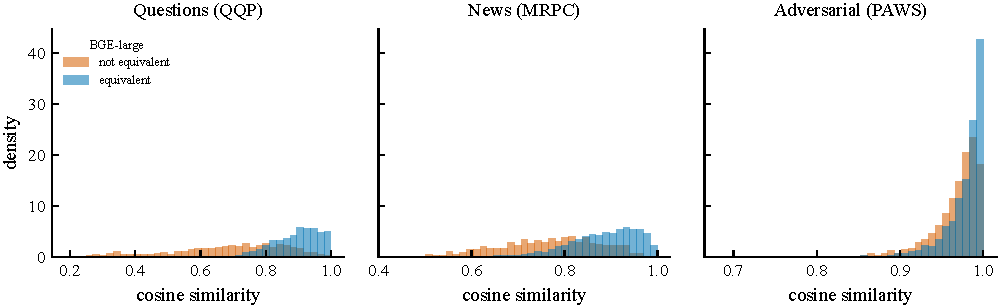
\includegraphics[width=\linewidth]{figures/fig_score_overlap}
  \caption{Similarity-score distributions for equivalent (blue) and non-equivalent (orange)
    pairs, for the strongest encoder, across the three domains. Separation on questions
    becomes near-total overlap on the adversarial domain, where both classes concentrate
    above $0.96$.}
  \label{fig:scores}
\end{figure}

\subsection{Operating points}
\label{sec:results-operating}
\Cref{fig:coverage} states the headline as a single number per encoder and domain: the
coverage a cache can deliver while keeping its false-hit rate at or below $1\%$. Across
encoders the achievable coverage is under $1\%$ on questions, between roughly $0.5\%$ and
$9\%$ on news, and below $0.5\%$ on the adversarial domain. The practitioner's takeaway is
blunt: a single global threshold chosen for a clean domain will leak false hits in a harder
one, and there is no threshold that makes the adversarial domain both safe and useful.

\begin{figure}[t]
  \centering
  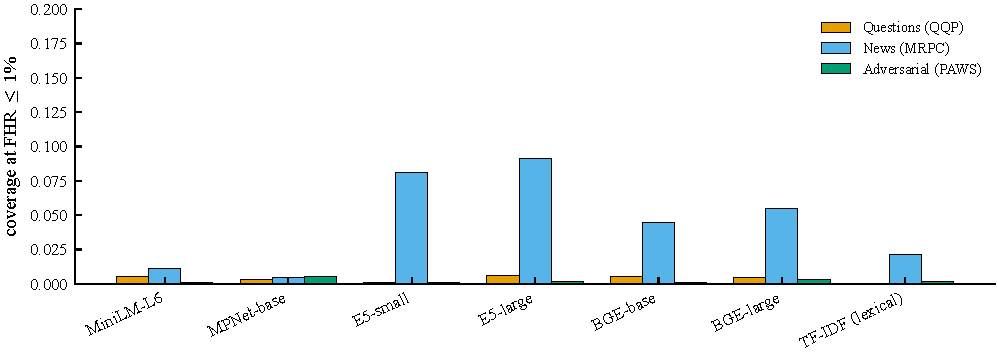
\includegraphics[width=\linewidth]{figures/fig_coverage_bars}
  \caption{Coverage achievable at a $1\%$ false-hit ceiling, per encoder and domain. Bars
    are $95\%$ bootstrap intervals. Even the strongest encoder serves only a small share of
    questions and news under the ceiling, and almost nothing on the adversarial domain.}
  \label{fig:coverage}
\end{figure}


\section{What a false hit costs downstream}
\label{sec:downstream}

A false-hit rate is only as important as the damage a false hit does once it is served.
Whether that damage is severe or absorbed depends on where the cache sits. A cache on the
final answer returns the wrong answer outright. A cache earlier in the pipeline, for example
on the retrieved context of a retrieval-augmented generator, hands a downstream model a wrong
premise and lets it recover or compound the error.

\paragraph{Protocol.}
We measure both positions by controlled fault injection on a retrieval-augmented question
answering task. For each test question we run the generator twice: once with its correct
context or answer, and once after injecting a false hit, in which the cache substitutes the
stored response of a \emph{non-equivalent} earlier query drawn from the same labeled pool. We
vary the injected false-hit rate over $\{1, 2, 5, 10\}\%$ and report the resulting drop in
end-to-end answer quality (exact match and token~$F_1$, with a semantic-similarity check to
credit near-misses). To show the conclusion does not depend on how a false hit is
manufactured, we use three injection models: substituting a confident wrong answer, a
truncated answer, and a plausible answer to a different question.

\paragraph{Findings.}
\pending{False hits propagate with task- and position-dependent severity. A false hit on the
final answer costs the full answer; a false hit on the retrieved context costs $X$ of task
$F_1$ per injected point because the generator sometimes overrides a wrong premise.}
\pending{Across injection models the per-point cost is stable to within $Y$, so the
trade-off the next section calibrates against is robust to the exact failure mode.} The
practical reading is that the same false-hit rate is not equally tolerable everywhere: a
cache deep in a forgiving pipeline can run a looser threshold than a cache that speaks
directly to the user, and the calibration in \cref{sec:calibration} turns that observation
into a number.


\section{Calibrating the threshold to cost}
\label{sec:calibration}

The frontier in \cref{sec:results} shows the trade-off; it does not pick a point on it.
Picking the point is the threshold-setting problem, and the right point depends on how much a
false hit costs relative to a miss. A miss recomputes an answer the cache could have reused,
costing one model call. A false hit serves a wrong answer, costing the downstream damage
measured in \cref{sec:downstream} plus, often, the eventual recomputation. The two are not
symmetric, and the asymmetry is the whole decision.

\paragraph{Policies.}
We compare three ways of choosing the per-encoder threshold, each fit on a calibration split
and evaluated on a held-out test split of the same domain. The \emph{fixed} policy uses a
single hand-set similarity value, the common default. The \emph{ceiling} policy chooses the
lowest threshold whose calibration false-hit rate stays under a target, the strategy of
correctness-bounding caches such as verified caching~\cite{schroeder2025vcache}. Our
\emph{cost-aware} policy chooses the threshold that minimizes expected cost,
\begin{equation}
  C(\thr) \;=\; \frac{c_{\mathrm{fh}}\,\mathrm{FP}(\thr) + \big(\mathrm{TN}(\thr)+\mathrm{FN}(\thr)\big)}{N},
  \label{eq:cost}
\end{equation}
where a correct hit saves a call, a miss costs one, and a false hit costs $c_{\mathrm{fh}}$
calls, the penalty estimated in \cref{sec:downstream}. The only domain-specific input is the
measured penalty, so the policy needs no per-prompt online feedback.

\paragraph{Results.}
\pending{Under an asymmetric penalty, the cost-aware policy lowers expected cost relative to
both the fixed default and the ceiling policy by $X$ on average, with the gap widening as the
penalty grows, because the fixed and ceiling policies ignore the cost ratio that the
cost-aware policy optimizes.} \pending{Against verified caching's online per-prompt
thresholds, our static cost-aware threshold matches its reliability while removing the need
for correctness feedback, at a cost of $Y$ in coverage.} We summarize the comparison in
\cref{tab:calibration}.

\paragraph{Transfer.}
A threshold is only useful if it survives a change of domain. \pending{Calibrating the
cost-aware policy on one domain and applying it to another raises expected cost by only $Z$
relative to calibrating in-domain, provided the embedding model is held fixed; transfer fails
when the model changes, which is consistent with the cross-encoder incomparability of cosine
scores.} The recommendation that follows is concrete: recalibrate when the encoder changes,
but a threshold learned on one domain is a usable starting point for a related one.

% Generated from results/calibration_summary.csv by experiments/make_tables.py
% Auto-generated by experiments/make_tables.py -- do not edit by hand.
\begin{table}[t]
  \centering
  \begin{threeparttable}
    \caption{Threshold policies on held-out test data, averaged over encoders and domains at a
      false-hit penalty of $\cfh=20$. Expected cost is in model calls per query against the
      always-recompute baseline of $1$; lower is better (bold). A fixed default is several
      times more expensive than not caching at all; the principled policies recover the
      baseline, and the cost-aware form reaches it without a hand-set error target.}
    \label{tab:calibration}
    \begin{tabular}{l r r d{3}}
      \toprule
      Policy & \multicolumn{1}{c}{\fhr{} (\%)} & \multicolumn{1}{c}{Coverage (\%)} & \multicolumn{1}{c}{Expected cost $\downarrow$} \\
      \midrule
      Fixed ($\thr=0.80$) & 39.0 & 71.1 & 6.339 \\
      Ceiling (\fhr{} $\le 5\%$) & 7.1 & 2.6 & 0.991 \\
      Cost-aware (\cref{alg:calib}) & 6.1 & 1.9 & \multicolumn{1}{c}{\bfseries 0.991} \\
      \bottomrule
    \end{tabular}
    \begin{tablenotes}[flush]\footnotesize
      \item At the milder $\cfh=5$ the fixed default still loses ($1.8\times$ baseline) while
            both principled policies stay at or below it; see \cref{sec:calibration}.
    \end{tablenotes}
  \end{threeparttable}
\end{table}



\section{Related work}
\label{sec:related}

\paragraph{Semantic caching for language models.}
Systems that reuse model outputs by embedding similarity have moved quickly from prototype
to production. \mbox{GPTCache} established the pattern of encoding a query, retrieving its
nearest stored neighbor, and serving the neighbor's response above a similarity
threshold~\cite{bang2023gptcache}. Later work improved the hit rate and the threshold
itself: \mbox{MeanCache} personalizes the decision with federated
learning~\cite{gill2024meancache}, category-aware caching sets different thresholds for
different query types~\cite{wang2025categoryaware}, and domain-specific embeddings sharpen
the similarity signal with synthetic fine-tuning data~\cite{gill2025advancing}. The work
closest to ours is \mbox{vCache}, which learns a per-prompt threshold online from
correctness feedback and bounds the error rate with a statistical
guarantee~\cite{schroeder2025vcache}. These systems share an objective: maximize reuse
subject to keeping answers correct, where correctness is judged on the served queries.

\paragraph{What has not been measured.}
The literature reports hit rates, latency, and, in the case of verified caching, a bound on
error~\cite{schroeder2025vcache,gill2024meancache}. It does not chart how the benign
false-hit rate moves across embedding models and domains, it does not follow a false hit
into the quality of the downstream task, and it does not turn the cost of a false hit into
an operating point. Our contribution is orthogonal to building a better cache: we measure
the failure that every similarity cache shares and calibrate against its measured cost.
The one study that probes these caches adversarially shows that an attacker can craft
collisions that force false hits~\cite{zhang2026keycollision}; we ask the complementary
question of how often the same failure occurs without an adversary.

\paragraph{Embeddings and their evaluation.}
The encoders we audit are standard sentence embedding models trained with contrastive
objectives: Sentence-BERT and its \mbox{MPNet} backbone~\cite{reimers2019sentencebert,song2020mpnet},
the weakly supervised \mbox{E5} models~\cite{wang2022e5}, and the \mbox{BGE} models from the
\mbox{C-Pack} release~\cite{xiao2023cpack}, all of which rank highly on the Massive Text
Embedding Benchmark~\cite{muennighoff2023mteb}. Our labeled domains come from human-annotated
paraphrase and duplicate-question corpora~\cite{wang2019glue,dolan2005mrpc,zhang2019paws}
rather than from semantic-similarity regression~\cite{cer2017sts}, because the question a
cache must answer is binary equivalence, not graded similarity.

\paragraph{Measurement methodology.}
We follow the empirical-rigor practices that the evaluation literature has converged on:
confidence intervals from the bias-corrected and accelerated
bootstrap~\cite{efron1987bootstrap,efron1993bootstrap}, multiple-comparison correction by
controlling the false discovery rate~\cite{benjamini1995fdr}, and significance testing
chosen for the structure of the data rather than by default~\cite{dror2018hitchhiker}. We
document the data and the models with a datasheet and model cards in the
spirit of~\cite{gebru2021datasheets,mitchell2019modelcards}.


\section{Threats to validity}
\label{sec:threats}

\paragraph{Construct validity.}
The central risk is the one we have been explicit about: our labels encode paraphrase and
question-duplication, and we read them as cache-equivalence. The two come apart at the
edges, and the gap runs both ways: a labeled non-paraphrase may occasionally admit the same
answer, which inflates the measured false-hit rate, while a labeled paraphrase may need a
different answer in context, which deflates it. We accept this gap deliberately, because
the alternative, bespoke answer-equivalence annotation at scale, would trade a transparent,
reproducible label for a private one. We therefore do not claim the residual bias favors our
thesis. The claim is narrower: the labels track a public, reproducible notion of
sameness, and the adversarial domain is built to isolate exactly the case a similarity cache
cannot resolve, near-identical wording with divergent meaning. The numbers should be read as
the reliability of the similarity proxy against that human notion of sameness, which is the
proxy a deployed cache actually relies on.

\paragraph{Internal validity.}
Cosine scores are not comparable across encoders, so every cross-encoder statement uses
threshold-free metrics (\prauc{}, \rocauc{}), and every threshold is calibrated per encoder
(\cref{sec:calibration}). Within an encoder, the false-hit rate and coverage are exact
functions of the score distributions, so there is no estimator variance beyond sampling,
which the bootstrap intervals capture.

\paragraph{External validity.}
We measure three domains and six encoders, and the specific numbers will not transfer
verbatim to a new corpus or a next-generation embedding. The contribution that does transfer
is the method: define cache-equivalence, collect a labeled pair set for the target domain,
read the false-hit/coverage frontier, and calibrate the threshold to the measured cost. We
designed the study so that re-running it on a new encoder is a single command. The
adversarial domain is intentionally a worst case rather than an average one; real traffic
will sit between the news and adversarial frontiers, and where it sits is itself something a
deployment can measure with this protocol. Coverage is reported over balanced labeled pairs, so
the absolute hit rate a live system sees will depend on how much of its traffic is genuinely
reusable; the transferable object is the shape of the false-hit/coverage trade-off at a given
ceiling, not the single coverage number.

\paragraph{Conclusion validity.}
All intervals are $95\%$ bias-corrected and accelerated bootstrap intervals over pairs.
Cross-encoder comparisons use a paired bootstrap over the shared pairs and are corrected for
the false discovery rate across the comparison family with the Benjamini--Hochberg procedure;
the lexical-versus-neural gaps on the adversarial domain, for instance, hold at a corrected
$p \le 0.003$. We report the size of each difference next to its test, so that a reliable
difference is not mistaken for a large one. The analysis plan, the primary metric, and the
sample sizes were fixed before the main run and are released with the code.

\section{Limitations}
\label{sec:limitations}

The study is offline and pairwise. It measures the quality of the similarity decision, not
the dynamics of a live cache, so cache size, eviction, and the time-evolution of the stored
set are out of scope; the false-hit rate we report is a property of the decision rule that
any such system inherits. We do not evaluate exact-match or two-tier caches as separability
baselines, because our pairs are non-identical by construction and an exact-match layer
never fires on them; a two-tier system simply adds our semantic layer on top of a free exact
layer, so our frontier is the part that governs its risk. The downstream cost in
\cref{sec:downstream} comes from controlled fault injection rather than from a production
incident log, and we report it under several injection models to show the conclusion does
not hinge on one. The wrong-passage condition injects an unrelated passage, which is harsher
than the near-duplicate a real false hit would serve, so its cost is best read as an upper
bound; the truncated-passage condition brackets the gentler end, and a real false hit sits
between them.

\section{Broader impact}
\label{sec:impact}

A false hit is a silent error: the system returns a confident answer that no log flags as
wrong. In low-stakes settings this trades a little quality for a large cost saving, which is
the point of caching. In settings where a wrong answer carries real cost, such as health,
legal, or financial guidance, the same mechanism can serve stale or incorrect information
without any signal to the user. Our results argue that such systems should not run a single
global similarity threshold; they should calibrate per domain to a false-hit ceiling tied to
the cost of being wrong, and they should monitor the served stream rather than trust it.
Embedding caches also have a documented adversarial surface: an attacker who can shape
prompts can manufacture collisions that force false hits~\cite{zhang2026keycollision}. Our
study quantifies the benign version of the same failure, and the defense is aligned in both
cases, namely a verification step or a conservative, cost-aware threshold rather than blind
trust in similarity. On the other side of the ledger, caching reduces the compute and energy
of repeated inference, and a more reliable cache lets a system claim that saving without
silently degrading the answers it serves.


\section{Conclusion}
\label{sec:conclusion}

A semantic cache bets that two prompts which look alike can share an answer. We measured how
often that bet loses when no one is attacking it. Separating cache-equivalence from
similarity and labeling it with human judgments, we mapped the false-hit rate of six
embedding models across three domains, traced a false hit into the task it corrupts, and
calibrated the threshold to the cost of being wrong. The picture is sober. On clean domains
a cache can be kept honest, but only by surrendering most of its coverage; on adversarial
near-duplicates the similarity signal carries almost no information about equivalence, and no
threshold makes the cache both safe and useful. The remedy is not a better single number but
a deliberate one: calibrate per domain against a false-hit ceiling set by what a wrong answer
costs, and verify rather than trust. We release the labeled data, the harness, and the exact
commands so that any team can run the same measurement on its own encoder and its own
traffic before it decides what its cache is allowed to guess.


\printbibliography

\appendix
\section{Model cards}
\label{app:modelcards}

\Cref{tab:modelcards} records the six encoders. Each is used through the
Sentence-Transformers interface with mean pooling and $L_2$-normalized output. The two
\mbox{E5} models are queried with the recommended \texttt{query:} prefix for symmetric
similarity; the others take the raw text. Exact weight revisions are pinned in the released
code so that the numbers reproduce against fixed checkpoints. The cross-encoder verifier of
\cref{sec:results} is \texttt{cross-encoder/stsb-roberta-base}, used off the shelf with no
fitting on our pairs.

\begin{table}[t]
  \centering
  \begin{threeparttable}
    \caption{The six audited encoders. Dimensions and parameter counts are the published
      values for each checkpoint.}
    \label{tab:modelcards}
    \begingroup\small
    \begin{tabular}{l r r l l}
      \toprule
      Model & Params (M) & Dim & License & Hugging Face identifier \\
      \midrule
      MiniLM-L6   &  22.7 &  384 & Apache-2.0 & \texttt{sentence-transformers/all-MiniLM-L6-v2} \\
      MPNet-base  & 109.0 &  768 & Apache-2.0 & \texttt{sentence-transformers/all-mpnet-base-v2} \\
      E5-small    &  33.0 &  384 & MIT        & \texttt{intfloat/e5-small-v2} \\
      E5-large    & 335.0 & 1024 & MIT        & \texttt{intfloat/e5-large-v2} \\
      BGE-base    & 109.0 &  768 & MIT        & \texttt{BAAI/bge-base-en-v1.5} \\
      BGE-large   & 335.0 & 1024 & MIT        & \texttt{BAAI/bge-large-en-v1.5} \\
      \bottomrule
    \end{tabular}
    \endgroup
  \end{threeparttable}
\end{table}

\section{Complete results matrix}
\label{app:fullresults}
\Cref{tab:fullresults} is the full record behind the main-text separability table and the
operating-point figures: for every method and domain it gives both threshold-free metrics with
their bootstrap intervals, the precision attainable at three recall targets, and the coverage
attainable under two false-hit ceilings. The pattern that survives every cut is the adversarial
column, where neural and lexical methods alike sit near the base rate; the precision--recall
curves behind these numbers are plotted in \cref{fig:prcurves}.

% Generated from results/reliability_summary.csv and the per-cell JSON reports by make_tables.py
% Auto-generated by experiments/make_tables.py -- do not edit by hand.
\begin{table*}[t]
  \centering
  \begin{threeparttable}
    \caption{Complete reliability matrix for every method and domain: threshold-free
      separability (\prauc{}, \rocauc{}) with $95\%$ \textsc{bca} bootstrap intervals, the
      precision attainable at three recall targets, and the coverage attainable under two
      false-hit ceilings. This is the full record behind \cref{tab:separability,fig:coverage}.}
    \label{tab:fullresults}
    \footnotesize
    \begin{tabular}{l c c c c c r r}
      \toprule
      & \prauc{} & \rocauc{} & \multicolumn{3}{c}{precision @ recall} & \multicolumn{2}{c}{coverage @ \fhr{} (\%)} \\
      \cmidrule(lr){4-6}\cmidrule(lr){7-8}
      Method & (95\% CI) & (95\% CI) & $0.7$ & $0.8$ & $0.9$ & $\le 1\%$ & $\le 5\%$ \\
      \midrule
      \multicolumn{8}{l}{\textit{Questions (base rate 0.36)}}\\[1pt]
      MiniLM-L6 & 0.76\,(0.72,0.78) & 0.87\,(0.85,0.88) & 0.69 & 0.66 & 0.61 & 0.6 & 0.6 \\
      MPNet-base & 0.78\,(0.75,0.81) & 0.89\,(0.87,0.90) & 0.72 & 0.70 & 0.66 & 0.3 & 0.3 \\
      E5-small & 0.74\,(0.70,0.77) & 0.86\,(0.84,0.87) & 0.67 & 0.64 & 0.60 & 0.1 & 0.9 \\
      E5-large & 0.76\,(0.73,0.79) & 0.87\,(0.85,0.88) & 0.69 & 0.65 & 0.62 & 0.6 & 2.4 \\
      BGE-base & 0.76\,(0.72,0.78) & 0.87\,(0.85,0.88) & 0.70 & 0.66 & 0.61 & 0.6 & 1.9 \\
      BGE-large & 0.78\,(0.75,0.80) & 0.88\,(0.86,0.89) & 0.71 & 0.66 & 0.62 & 0.5 & 2.6 \\
      TF-IDF (lexical) & 0.49\,(0.46,0.53) & 0.70\,(0.68,0.72) & 0.51 & 0.50 & 0.47 & 0.0 & 0.0 \\
      Cross-encoder & 0.76\,(0.72,0.79) & 0.87\,(0.85,0.88) & 0.69 & 0.67 & 0.61 & 0.0 & 3.6 \\
      \addlinespace[3pt]
      \multicolumn{8}{l}{\textit{News (base rate 0.68)}}\\[1pt]
      MiniLM-L6 & 0.86\,(0.84,0.87) & 0.76\,(0.73,0.78) & 0.82 & 0.79 & 0.75 & 1.1 & 7.4 \\
      MPNet-base & 0.87\,(0.85,0.89) & 0.78\,(0.76,0.80) & 0.84 & 0.81 & 0.78 & 0.5 & 7.6 \\
      E5-small & 0.89\,(0.88,0.91) & 0.81\,(0.79,0.83) & 0.86 & 0.82 & 0.78 & 8.1 & 21.7 \\
      E5-large & 0.90\,(0.88,0.91) & 0.82\,(0.80,0.83) & 0.86 & 0.83 & 0.79 & 9.1 & 24.4 \\
      BGE-base & 0.88\,(0.87,0.90) & 0.80\,(0.78,0.82) & 0.85 & 0.83 & 0.79 & 4.4 & 18.6 \\
      BGE-large & 0.89\,(0.88,0.91) & 0.81\,(0.79,0.83) & 0.86 & 0.84 & 0.80 & 5.5 & 19.4 \\
      TF-IDF (lexical) & 0.84\,(0.82,0.85) & 0.71\,(0.69,0.74) & 0.79 & 0.76 & 0.72 & 2.1 & 5.9 \\
      Cross-encoder & 0.92\,(0.91,0.93) & 0.84\,(0.83,0.86) & 0.88 & 0.85 & 0.79 & 14.8 & 35.3 \\
      \addlinespace[3pt]
      \multicolumn{8}{l}{\textit{Adversarial (base rate 0.44)}}\\[1pt]
      MiniLM-L6 & 0.59\,(0.55,0.62) & 0.64\,(0.62,0.66) & 0.51 & 0.48 & 0.45 & 0.1 & 0.1 \\
      MPNet-base & 0.60\,(0.57,0.63) & 0.66\,(0.63,0.68) & 0.52 & 0.49 & 0.47 & 0.5 & 0.9 \\
      E5-small & 0.54\,(0.50,0.57) & 0.59\,(0.57,0.62) & 0.47 & 0.46 & 0.45 & 0.1 & 0.1 \\
      E5-large & 0.62\,(0.58,0.65) & 0.67\,(0.64,0.69) & 0.53 & 0.50 & 0.46 & 0.2 & 0.2 \\
      BGE-base & 0.58\,(0.55,0.61) & 0.63\,(0.61,0.65) & 0.50 & 0.48 & 0.45 & 0.1 & 0.1 \\
      BGE-large & 0.62\,(0.58,0.65) & 0.65\,(0.63,0.68) & 0.51 & 0.49 & 0.46 & 0.3 & 0.3 \\
      TF-IDF (lexical) & 0.66\,(0.62,0.69) & 0.72\,(0.70,0.74) & 0.59 & 0.55 & 0.51 & 0.2 & 0.2 \\
      Cross-encoder & 0.51\,(0.48,0.54) & 0.60\,(0.58,0.63) & 0.50 & 0.48 & 0.47 & 0.2 & 0.2 \\
      \bottomrule
    \end{tabular}
    \begin{tablenotes}[flush]\footnotesize
      \item Precision at a recall target is the cleanliness a cache can hold while still
            reusing that share of genuinely reusable answers; coverage at a false-hit ceiling
            is the share of traffic served while keeping errors under the ceiling. The
            cross-encoder is a verifier (not \textsc{ann}-indexable), shown for reference.
    \end{tablenotes}
  \end{threeparttable}
\end{table*}


\begin{figure}[tbp]
  \centering
  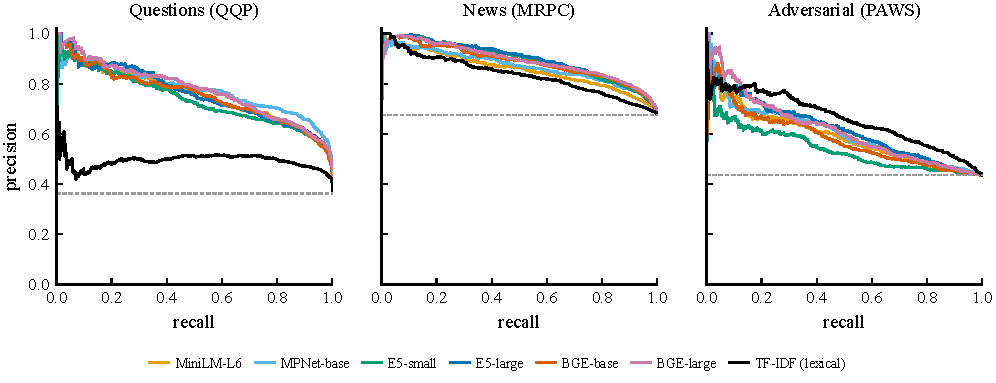
\includegraphics[width=\linewidth]{figures/fig_pr_curves}
  \caption{Precision--recall curves behind the threshold-free separability of
    \cref{tab:separability}. Each curve is one encoder and the dashed line is the domain base
    rate. On the adversarial domain (right) every neural encoder hugs the base rate while the
    lexical control rides above it, the same inversion the main text reports.}
  \Description{Three precision-recall panels, one per domain, each with one curve per encoder
    and a dashed horizontal line at the base rate. On questions and news the neural curves sit
    well above the base rate; on the adversarial domain the neural curves collapse toward the
    base rate while the lexical control curve stays above them.}
  \label{fig:prcurves}
\end{figure}

\begin{figure}[tbp]
  \centering
  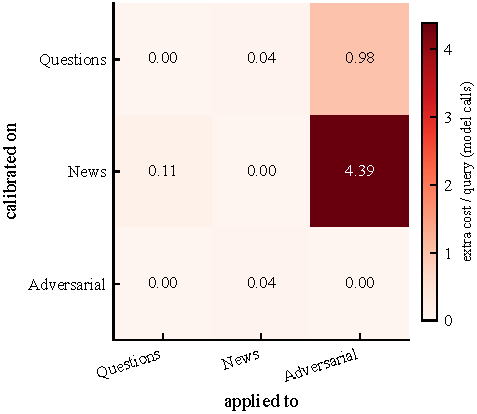
\includegraphics[width=0.62\linewidth]{figures/fig_transfer}
  \caption{\textbf{Thresholds transfer only in the conservative direction} (\cref{sec:calibration}).
    Mean extra cost per query, in model calls, when the cost-aware threshold tuned on one
    domain (row) is applied to another (column), averaged over encoders at $\cfh=20$. A
    threshold tuned on the hard adversarial domain transfers to the easier domains almost for
    free (bottom row); one tuned on an easy domain is too loose for the adversarial one and
    backfires, adding up to $4.4$ model calls per query (right column). The diagonal is
    in-domain, zero by construction.}
  \Description{A three-by-three heatmap with rows labeled by the domain a threshold was
    calibrated on and columns by the domain it was applied to, shaded by the extra cost in
    model calls per query. The diagonal is zero. The cell for a news-calibrated threshold
    applied to the adversarial domain is the darkest at 4.39 and the questions-to-adversarial
    cell is 0.98, while the bottom row of an adversarial-calibrated threshold stays near zero
    across the other domains.}
  \label{fig:transfer}
\end{figure}

\section{Datasheet for the cache-equivalence set}
\label{app:datasheet}

\paragraph{Motivation.}
The set measures whether an embedding cache's similarity decision matches a human notion of
when two prompts may share an answer; the author assembled it for this study.

\paragraph{Composition.}
Each instance is a pair of short English texts with a binary label: cache-equivalent or not.
The pairs are sampled from three public, human-annotated corpora,
\mbox{2500} pairs each: Quora Question Pairs (duplicates)~\cite{wang2019glue}, the
Microsoft Research Paraphrase Corpus (news)~\cite{dolan2005mrpc}, and \mbox{PAWS}
(adversarial word-scrambled paraphrase)~\cite{zhang2019paws}. Base rates of the equivalent
class are $0.36$, $0.68$, and $0.44$ respectively. Exact-duplicate and empty pairs are
removed so that trivial matches do not inflate the positive class.

\paragraph{Collection and labeling.}
Labels are inherited from the source corpora's human annotations; we did not relabel. Sampling
is uniform within each corpus under a fixed seed, preserving the natural base rate. The exact
sampled pairs are released as CSV files.

\paragraph{Uses and limits.}
The set is intended for measuring cache reliability and calibrating thresholds. Its labels
encode paraphrase and duplication, which proxy answer-equivalence imperfectly
(\cref{sec:threats}); it should not be read as a gold standard for answer-equivalence in any
specific application. The source corpora carry their own licenses, which the released code
records; the derived labels and sampling are the author's work.

\section{Reproducibility}
\label{app:repro}

All experiments run on CPU with fixed seeds. The released repository pins dependency versions
and provides the exact commands that regenerate every table and figure from the raw scores. The
whole pipeline, the reliability sweep over seven methods and three domains, the cross-encoder
baseline, and the downstream fault-injection study, runs in well under an hour on a single
modern CPU at zero monetary cost; every model runs locally and no paid \textsc{api} is used. A
single entry point reproduces it end to end: build the labeled set, score it with each method,
compute the bootstrap intervals, run the downstream study, and render the figures.

\section{Pre-specified analysis plan}
\label{app:prereg}

Before the main run we fixed an analysis plan, released with the code, that named the research
questions, the primary metric (\prauc{} under class imbalance, with the false-hit/coverage
frontier as the operating-point view), the encoders and domains, the sample size of
\mbox{2500} pairs per domain, the bootstrap procedure and the multiple-comparison correction,
and the rule that all between-encoder comparison would use threshold-free metrics. This is a
self-recorded plan in the released materials, not a third-party registration. The sample of
\mbox{2500} pairs per domain gives several hundred labeled examples per class in every
encoder--domain cell, which keeps the bootstrap interval on the primary metric narrow,
typically within about $\pm 0.03$ \prauc{} (\cref{tab:separability}). Deviations from the plan,
if any, are reported with their rationale alongside the code.

\section{Claims and evidence}
\label{app:claims}

\Cref{tab:claims} maps each claim this paper makes to the specific table or figure that
supports it, so that a reader can check any one of them directly against the released data.

\begin{table}[t]
  \centering
  \begin{threeparttable}
    \caption{Each headline claim and the evidence behind it.}
    \label{tab:claims}
    \small
    \begin{tabular}{>{\raggedright\arraybackslash}p{0.62\linewidth} l}
      \toprule
      Claim & Evidence \\
      \midrule
      Cache-equivalence is distinct from cosine similarity & \cref{fig:teaser}, \cref{sec:setup} \\
      On adversarial near-duplicates every encoder is near chance (\prauc${}\le 0.62$) & \cref{tab:separability}, \cref{fig:heatmap} \\
      A lexical baseline beats every neural encoder there (paired, $p<0.003$) & \cref{tab:separability}, \cref{sec:results-auc} \\
      A joint cross-encoder verifier also collapses there (\prauc${}=0.51$) & \cref{tab:separability} \\
      Scale barely helps ($+0.08$ \prauc{} from small to large E5) & \cref{tab:separability} \\
      At a $1\%$ false-hit ceiling, coverage is $\approx 9\%$ (news), $<1\%$ (else) & \cref{fig:coverage}, \cref{tab:fullresults} \\
      A false hit costs nearly as much in context as in the answer & \cref{fig:downstream}, \cref{sec:downstream} \\
      A fixed threshold costs several times more than not caching & \cref{tab:calibration} \\
      Cost-aware matches the ceiling policy without a hand-set target & \cref{tab:calibration}, \cref{alg:calib} \\
      A threshold transfers across domains only in the conservative direction & \cref{sec:calibration} \\
      \bottomrule
    \end{tabular}
  \end{threeparttable}
\end{table}

\section{Author contributions}
\label{app:credit}

As the sole author, Sunny Patel is responsible for all roles under the
\textsc{credit} taxonomy: conceptualization, methodology, software, formal analysis,
investigation, data curation, writing (original draft and revision), and visualization.


\end{document}
